%
% This is a borrowed LaTeX template file for lecture notes for CS267,
% Applications of Parallel Computing, UCBerkeley EECS Department.
% Now being used for CMU's 10725 Fall 2012 Optimization course
% taught by Geoff Gordon and Ryan Tibshirani.  When preparing 
% LaTeX notes for this class, please use this template.
%
% To familiarize yourself with this template, the body contains
% some examples of its use.  Look them over.  Then you can
% run LaTeX on this file.  After you have LaTeXed this file then
% you can look over the result either by printing it out with
% dvips or using xdvi. "pdflatex template.tex" should also work.
%

\documentclass[twoside]{article}
\setlength{\oddsidemargin}{0.25 in}
\setlength{\evensidemargin}{-0.25 in}
\setlength{\topmargin}{-0.6 in}
\setlength{\textwidth}{6.5 in}
\setlength{\textheight}{8.5 in}
\setlength{\headsep}{0.75 in}
\setlength{\parindent}{0 in}
\setlength{\parskip}{0.1 in}

%
% ADD PACKAGES here:
%

\usepackage{amsmath,amsfonts,graphicx}

%
% The following commands set up the lecnum (lecture number)
% counter and make various numbering schemes work relative
% to the lecture number.
%
\newcounter{lecnum}
\renewcommand{\thepage}{\thelecnum-\arabic{page}}
\renewcommand{\thesection}{\thelecnum.\arabic{section}}
\renewcommand{\theequation}{\thelecnum.\arabic{equation}}
\renewcommand{\thefigure}{\thelecnum.\arabic{figure}}
\renewcommand{\thetable}{\thelecnum.\arabic{table}}

%
% The following macro is used to generate the header.
%
\newcommand{\lecture}[4]{
   \pagestyle{myheadings}
   \thispagestyle{plain}
   \newpage
   \setcounter{lecnum}{#1}
   \setcounter{page}{1}
   \noindent
   \begin{center}
   \framebox{
      \vbox{\vspace{2mm}
    \hbox to 6.28in { {\bf UCSB CS 291D: Blockchains and Cryptocurrencies
	\hfill Fall 2020} }
       \vspace{4mm}
       \hbox to 6.28in { {\Large \hfill Lecture #1: #2  \hfill} }
       \vspace{2mm}
       \hbox to 6.28in { {\it Lecturer: #3 \hfill Scribes: #4} }
      \vspace{2mm}}
   }
   \end{center}
   \markboth{Lecture #1: #2}{Lecture #1: #2}

%   {\bf Note}: {\it LaTeX template courtesy of UC Berkeley EECS dept.}

%   {\bf Disclaimer}: {\it These notes have not been subjected to the
%   usual scrutiny reserved for formal publications.  They may be distributed
%   outside this class only with the permission of the Instructor.}
%   \vspace*{4mm}
}
%
% Convention for citations is authors' initials followed by the year.
% For example, to cite a paper by Leighton and Maggs you would type
% \cite{LM89}, and to cite a paper by Strassen you would type \cite{S69}.
% (To avoid bibliography problems, for now we redefine the \cite command.)
% Also commands that create a suitable format for the reference list.
\renewcommand{\cite}[1]{[#1]}
\def\beginrefs{\begin{list}%
        {[\arabic{equation}]}{\usecounter{equation}
         \setlength{\leftmargin}{2.0truecm}\setlength{\labelsep}{0.4truecm}%
         \setlength{\labelwidth}{1.6truecm}}}
\def\endrefs{\end{list}}
\def\bibentry#1{\item[\hbox{[#1]}]}

%Use this command for a figure; it puts a figure in wherever you want it.
%usage: \fig{NUMBER}{SPACE-IN-INCHES}{CAPTION}
\newcommand{\fig}[3]{
			\vspace{#2}
			\begin{center}
			Figure \thelecnum.#1:~#3
			\end{center}
	}
% Use these for theorems, lemmas, proofs, etc.
\newtheorem{theorem}{Theorem}[lecnum]
\newtheorem{lemma}[theorem]{Lemma}
\newtheorem{proposition}[theorem]{Proposition}
\newtheorem{claim}[theorem]{Claim}
\newtheorem{corollary}[theorem]{Corollary}
\newtheorem{definition}[theorem]{Definition}
\newenvironment{proof}{{\bf Proof:}}{\hfill\rule{2mm}{2mm}}

% **** IF YOU WANT TO DEFINE ADDITIONAL MACROS FOR YOURSELF, PUT THEM HERE:

\newcommand\E{\mathbb{E}}

\begin{document}
%FILL IN THE RIGHT INFO.
%\lecture{**LECTURE-TITLE**}{**DATE**}{**LECTURER**}{**SCRIBE**}
\lecture{6}{Etherenm and EVM}{Shumo Chu}{Zuying Hu, Sanjay Chandrasekaran
}
%\footnotetext{These notes are partially based on those of Nigel Mansell.}

% **** YOUR NOTES GO HERE:

% Some general latex examples and examples making use of the
% macros follow.  
%**** IN GENERAL, BE BRIEF. LONG SCRIBE NOTES, NO MATTER HOW WELL WRITTEN,
%**** ARE NEVER READ BY ANYBODY.
%This lecture's notes illustrate some uses of
%various \LaTeX\ macros.  
%Take a look at this and imitate.

\section{Smart Contract} % Don't be this informal in your notes!
We have learned how to reach a consensus. Based on consensus and blockchain, we could build up a decentralized payment system. Moreover, we could apply consensus into much more complex  situations. For example, Alice wants to buy a computer from Bob, but Alice and Bob are geographically apart from each other. Alice wants to pay Bob, but there is a risk if Alice pays first then Bob may never send the computer to Alice. Can we build up a contract such that Alice and Bob could make this deal?

%What if Alice first makes the payment but then Bob refuses to ship the computer to her?
%\begin{lemma}
%This is the first lemma of the lecture.
%\end{lemma}

%\begin{proof}
%The proof is by induction on $\ldots$.
%For fun, we throw in a figure.
%%%NOTE USAGE !
%\fig{1}{1in}{A Fun Figure}

%This is the end of the proof, which is marked with a little box.
%\end{proof}

\subsection{Hash Time Lock Contract}
Naive contract: Alice sends 1 BTC to Bob in the form of UTXO which is controlled by a script. To make the payment successful, Alice needs to commit this script where the destination address should be same as Bob's. Then Bob could spend this UTXO as he wants. However, one flaw of this contract is that Bob could refuse to ship the computer after he receives the BTC.
To avoid this problem, ideally, Bob's spending of the UTXO should be conditioned on Bob's shipment of the computer. In reality, Bob's spending of the UTXO could be conditioned on Alice's ACK of the shipment. To achieve this, Alice first generate a secrete key: $S \xleftarrow[]{\$ } D , H(s)$, and UTXO is spendable for Bob based on two requirements:
\begin{enumerate}
\item The address is Bob's;
\item Bob provides secrete $S$, s.t. $H(S) = \nu$, $\nu$ is embedded in the script.
\end{enumerate}
When paying for the computer, Alice generates the secret key $S$ but does not give it to Bob immediately. After Alice commits the script, Bob could verify the address is his and then ship the computer. After receiving the computer, Alice could send the secrete $S$ to Bob. Then Bob could spend this UTXO. 
However, there still exist another risk: Bob could refuse to ship the computer even after Alice has committed the script. In this case, Alice's money is locked and can not get it back, and Bob can not get the money either, causing the bitcoin to be lost forever. Therefore, the third requirement is introduced:
\begin{enumerate}
\setcounter{enumi}{2}
\item After a period of T, Alice can take back this UTXO if Bob does not claim it.
\end{enumerate}
Up to now we have built up a contract called Hash Time Lock Contrat (HTLC) where UTXO is only spendable for Bob based on three requirements.
But HTLC is also a faulty scheme. Alice could also refuse to send ACK or the secret key $S$ even after she has received the computer. Hence, a 3-rd party should be introduced in this scheme to force both Alice and Bob to comply with the rules. The 3-rd party would receive secret key from Alice before telling Bob to ship the computer. Once Alice acknowledges she has received the computer the 3-rd party will deliver the secret key to Bob. In the case of a dispute where Alice claims to not receive the computer after Bob claims to have shipped it, it is up to the 3-rd party to decide whether Bob will receive the money or Alice will receive her money back.

\subsection{Limitations of bitcoin script}
HTLC is achievable by bitcoin script programming. However, there are some applications where it's hard or even impossible to use bitcoin script programming.
\begin{itemize}
\item App 1: Cryptographic Wallet which manages UTXOs for a user. Wallet has a $RootKey(Pk_r, Sk_r)$ denoted as $\lambda$ which controls multiple UTXOs. Users can't enforce a policy that only two BTCs could be transfered per day among these UTXOs. At any given time our BTC can be involved a number of UTXOs. When specifying some UTXO in a transaction, we are unable to condition whether this is over the two BTC daily limit, because it involves information from other UTXOs on the blockchain.
\item App 2: DNS on blockchain [ucsb.edu $\rightarrow$ IP] which has such functions: New(addr, name), Lookup(name), Update(name, newVal, newOwner, Sig). Trying to use bitcoin script to encode these functions could fail for lack of the ability to inspect the global state of consensus. For example, two entities could both attempt to register the same domain.
\end{itemize}
\subsection{Ethereum}
Ethereum \cite{1} came out as a platform to natively support general smart contract on blockchain. Ethereum could be applied in many decentralized applications (DAPP) such as 1) new coins(ERC-20). 2) decentralized finance(DeF) including exchanges, lending, stable coins and derivatives. 3) insurance. 4) asset based games like CryptoKitty. 5) distinguished asset (ERC-821).\\
Before going into the details about Ethereum, let's recall bitcoin state transition first as seen in figure \ref{fig Bitcoin state transition}. Coins in UTXOs are immutable, meaning that they cannot be modified. Old coins are destroyed when new coins are created in transactions.
\begin{figure}[h]
\centering
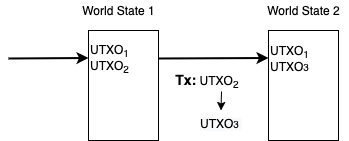
\includegraphics[width=6cm]{fig_1.png}
\caption{Bitcoin state transition}
\label{fig Bitcoin state transition}
\end{figure}

Ethereum state transition is shown in figure \ref{fig ethereum state transition}. From a high level overview, this transition contains two layers:
\begin{itemize}
\item Layer 1: consensus (global state)
\item Layer 1.5: computation which must be deterministic and subjective (to reach a consensus)
\end{itemize}

\begin{figure}[h]
\centering
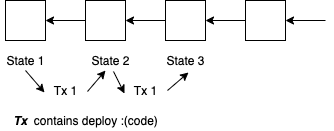
\includegraphics[width=6cm]{fig_2.png}
\caption{Ethereum state transition}
\label{fig ethereum state transition}
\end{figure}

Ethereum consensus protocol: 1) a variant of Nakamote (Pow). 2) avg. block rate is about 15 sec. 3) 150 Txn per block. 4). BlockReward: 2ETH + Txn Fee

For Ethereum computation, world state is a set of accounts with 160 bits address and associated data. Two types of accounts: 1) owned: ECDSA key pair ($Pk$, $Sk$). 2) contract account controlled by code which cannot be changed. Contract account could only be created by owned account. The data format for these two account is shown in figure \ref{fig account data format}.
\begin{figure}[h]
\centering
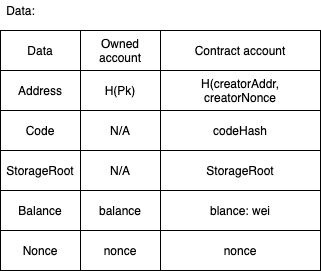
\includegraphics[width=6cm]{fig_3.png}
\caption{Account Data Format (wei named with Wei Dai, $10^{18}~wei = 1~ETH$)}
\label{fig account data format}
\end{figure}

Nonce = (\# of Txn send) + (\# of account created). Nonce is an unique identifier for the given type since nonce is monotonically increased. Each account is associates with a persistent storage which is an array of an account: S[0,...,$2^{256} - 1$] with each entry of 32 bytes. StorageRoot is a Merkle root (Merkle Patricia Trie) of this array.

After finishing Ethereum state transition, let's focus on Ethereum Txn and Msg. Txn is signed by initiator and contains: 1) To and From: 32-byte addr (if the account is new created, To = 0). 2) Signature. 3) Value of ETH transferred. 4) gasPrice and gasLimit (maximum gas user could spend). For example, if pricePrice = 3 wei and gasLimit = 3000 then one could spend at most 9,000 wei. One could get the gas back. If gas is not ran out of, one could also get the gas back. But if the gasPrice is not attractive, no miner will take this transaction. 5) case 1: To = 0, code = (init, body); case 2: To $\neq$ 0, data = (Function, arguments). 6) nonce. Nonce could ensure that one Txn appears only once. If Alice's current nonce is 4 and the Txn succeeds, her nonce will become 5. There are two types of Txn: owned $\rightarrow$ owned, owned $\rightarrow$ contract. 

In Ethereum, Msg is a virtual Txn initiated by a contract: contract $\rightarrow$ owned, contract $\rightarrow$ contract. Msg must be triggered by a Txn from a user. With this design a chain of Txn and Msg could be generated. A single Txn could lead a series of Msgs and the global state won't changed by this Txn even when only one msg failed. An example is shown in figure \ref{fig example}.
\begin{figure}[h]
\centering
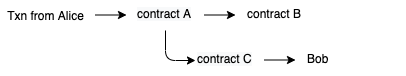
\includegraphics[width=8cm]{fig_4.png}
\caption{Example}
\label{fig example}
\end{figure}

Here is an example of application of Ethereum. For example, we have SBCoin, then we could build up a contract and some functions like \emph{func new()}, \emph{func payment()}.
\begin{tabbing}
\hspace*{.25in} \= \hspace*{.25in} \= \hspace*{.25in} \= \hspace*{.25in} \= \hspace*{.25in} \=\kill
\>{\bf Contract SBCoin} \{ \\
\>\> Struct SBEntry\{ \\
\>\>\> address: Owner\\
\>\>\> byte32: Val\\
\>\>\}\\
\>\>mapping(byte32 $\Rightarrow$ SBEntry): Data;\\
\> \}
\end{tabbing}
%
%Here is an itemized list:
%\begin{itemize}
%\item this is the first item;
%\item this is the second item.
%\end{itemize}

%Here is an enumerated list:
%\begin{enumerate}
%\item this is the first item;
%\item this is the second item.
%\end{enumerate}

%Here is an exercise:

%{\bf Exercise:}  Show that ${\rm P}\ne{\rm NP}$.

%Here is how to define things in the proper mathematical style.
%Let $f_k$ be the $AND-OR$ function, defined by

%\[ f_k(x_1, x_2, \ldots, x_{2^k}) = \left\{ \begin{array}{ll}

%	x_1 & \mbox{if $k = 0$;} \\
%
%	AND(f_{k-1}(x_1, \ldots, x_{2^{k-1}}),
%	   f_{k-1}(x_{2^{k-1} + 1}, \ldots, x_{2^k}))
%	 & \mbox{if $k$ is even;} \\
%
%	OR(f_{k-1}(x_1, \ldots, x_{2^{k-1}}),
%	   f_{k-1}(x_{2^{k-1} + 1}, \ldots, x_{2^k}))	
%	& \mbox{otherwise.} 
%	\end{array}
%	\right. \]

%\begin{theorem}
%This is the first theorem.
%\end{theorem}

%\begin{proof}
%This is the proof of the first theorem. We show how to write pseudo-code now.
%*** USE PSEUDO-CODE ONLY IF IT IS CLEARER THAN AN ENGLISH DESCRIPTION

%Consider a comparison between $x$ and~$y$:

%This concludes the proof.
%\end{proof}


%\section{Next topic}

%Here is a citation, just for fun~\cite{CW87}.

\section*{References}
\beginrefs
\bibentry{1}{\sc{DR. GAVIN WOOD}}, 
''ETHEREUM: A SECURE DECENTRALISED GENERALISED TRANSACTION LEDGER''

\endrefs

% **** THIS ENDS THE EXAMPLES. DON'T DELETE THE FOLLOWING LINE:

\end{document}

